\section{\acf{OPL} / \acf{HQ}}
\begin{wrapfigure}{r}{0.5\textwidth}
	\centering 
	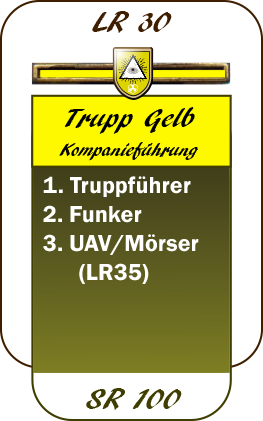
\includegraphics[width=0.35\textwidth]{./img/truppenordnung/opl/opl.png}
	\caption{Beispiel einer \ac{OPL}}
\end{wrapfigure}	

Die \ac{OPL} ist die höchste Instanz innerhalb einer Mission. Sie hat den Oberbefehl über alle Einheiten inne, koordiniert das allgemeine Vorgehen innerhalb der Mission und verwaltet die Zuordnung der unterstützenden Einheiten zu den kämpfenden Einheiten.Sie kommuniziert grundsätzlich nur über die Long-Range mit ihren untergeordneten Einheiten.\\
Die \ac{OPL} ist folgendermaßen aufgebaut:
\begin{itemize}
	\item Operationsleiter/\acs{OPL} (\acf{CO}): Der Oberbefehlshaber der Mission. Er gibt die Befehle und erstellt "den großen Plan".
	\item stellv. \ac{OPL} (\acf{XO}): Unterstützt den \ac{OPL} bei seinen Aufgaben, typischerweise beim Funken mit den untergeordneten Trupps. Kann jedoch auch alle weiteren Aufgaben übernehmen, die ihm der \ac{OPL} überträgt - er ist Mädchen für alles. Bewährt hat sich das Prinzip, dass der \ac{OPL} den eingehenden Funk übernimmt (Anfragen von anderen Trupps) und der stellv. \ac{OPL} den ausgehenden Funk (Abfragen von Statusberichten, Übermittlung von neuen Befehlen).
\end{itemize}
Ergänzt werden kann die \ac{OPL} durch maximal 4 Spieler, welche folgende Rollen einnehmen können:
\begin{itemize}
	\item Funker (\acf{RO}): ein zusätzlicher Funker, um die \ac{OPL} zu unterstützen, kann auf eine Spezialrolle beschränkt sein und für diese eine eigene LR-Frequenz bekommen (so kann es z.B. bei einer Mission mit vielen Lufteinheiten sinnvoll sein, jemanden zu haben, der sich auf einer eigenen Frequenz nur um die Koordination der Lufteinheiten um das Flugfeld kümmert und zentraler Ansprechpartner aller Lufteinheiten für Start-/Landemanöver ist)
	\item Aufklärungsoffizier (\acf{IO}): Sammelt alle verfügbaren, relevanten Daten und leitet diese gegebenenfalls an andere Trupps weiter. Hat meistens eine eigene, "große" Drohne (Greyhawk/Global Hawk) zur Feindaufklärung.
	\item freie Rolle (maximal einmal): je nach Mission kann es sinnvoll sein, dem \ac{OPL} einen Sanitäter, einen Nahsicherer, einen Fahrer o.Ä. zur Seite zu stellen
\end{itemize}
Je nach Größe und Struktur der Mission kann die \ac{OPL} identisch sein mit
\begin{itemize}
	\item der Sektionsführung, falls die Truppstruktur der Mission nur aus einer Sektion besteht
	\item der Zugführung, falls die Truppstruktur der Mission nur aus einem Zug besteht (egal ob Infanteriezug, Panzerzug oder mechanisierte Infanterie). Dies ist die einzige Ausnahme, in der die \ac{OPL} per Short-Range statt Long-Range mit ihren untergeordneten Einheiten kommuniziert.
\end{itemize}
Die OPL hält typischerweise einen sehr großen Abstand zu ihren Truppen - oft bleibt sie auch durchgehend in der Basis.